\chapter{BANG/BANG} 
\label{sec:bangbang}
\lstset{style=6502Style}

\vspace{-3.0cm}
\begin{figure}[H]
    \hspace{2cm}
    \begin{adjustbox}{width=9cm,center}
      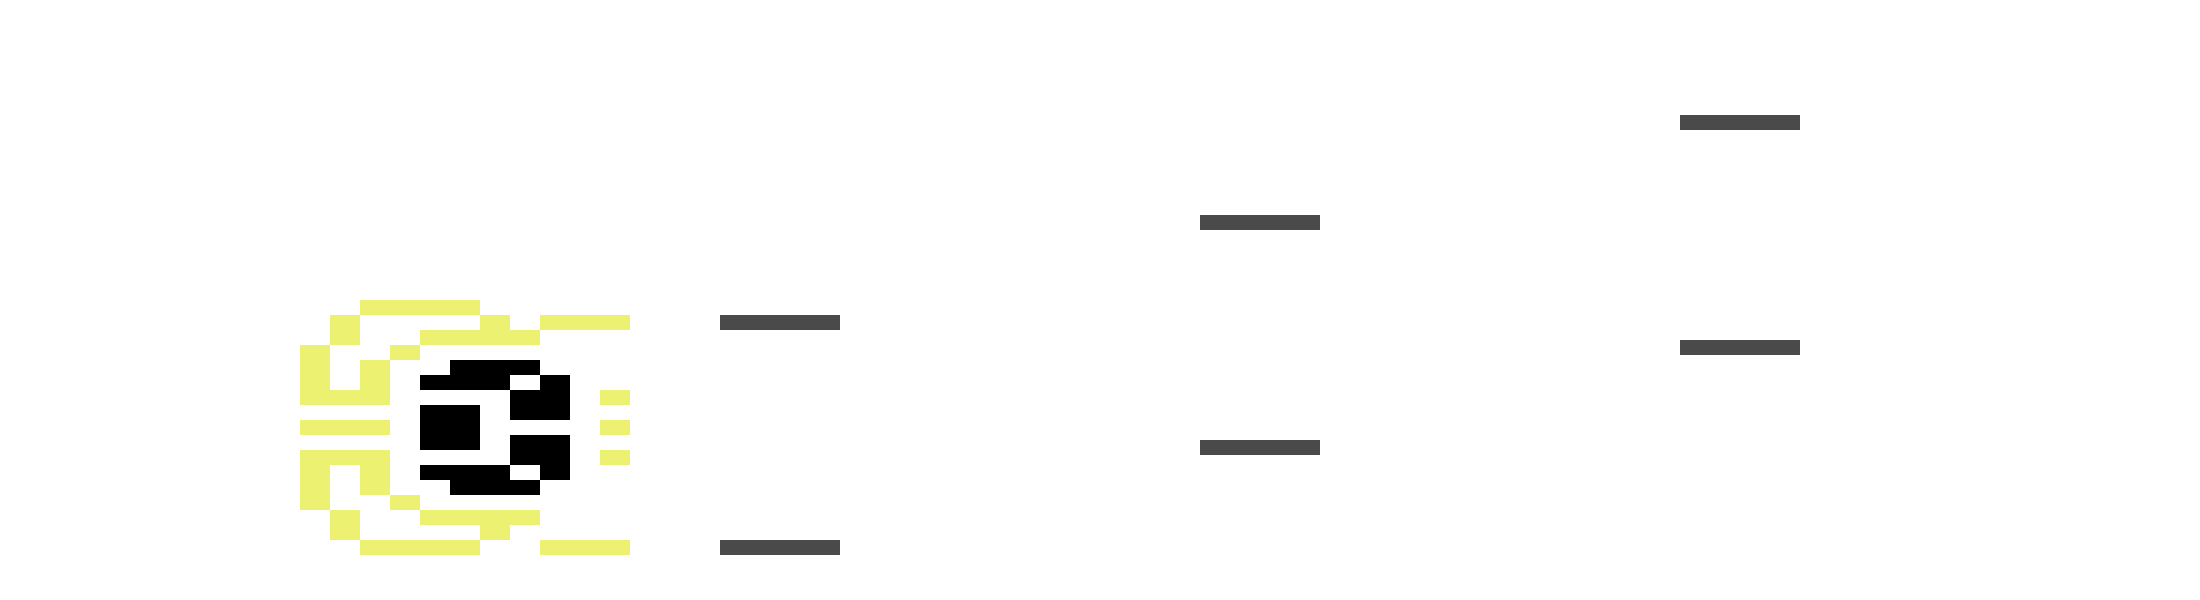
\includegraphics{src/bullets_player/bullets.png}%
    \end{adjustbox}
\end{figure}
\vspace{-0.4cm}


We can learn quite a lot about how the player's bullets are implemented in Uridium by
observing the frame by frame evolution of a bullet being fired across the deck at a 
static feature on the dreadnought. To aid us in our understanding, I've placed a grid
over the diagram so that we can tell where the character boundaries are in the character
set that makes up the surface of the dreadnought.

When the player presses fire, two bullets appear next to the Manta's cannons. We notice
that the bullets are exactly one character wide and confined to the cells in the character
grid that are nearest to the Manta.
\begin{figure}[H]
    \begin{adjustbox}{width=13.2cm,left}
      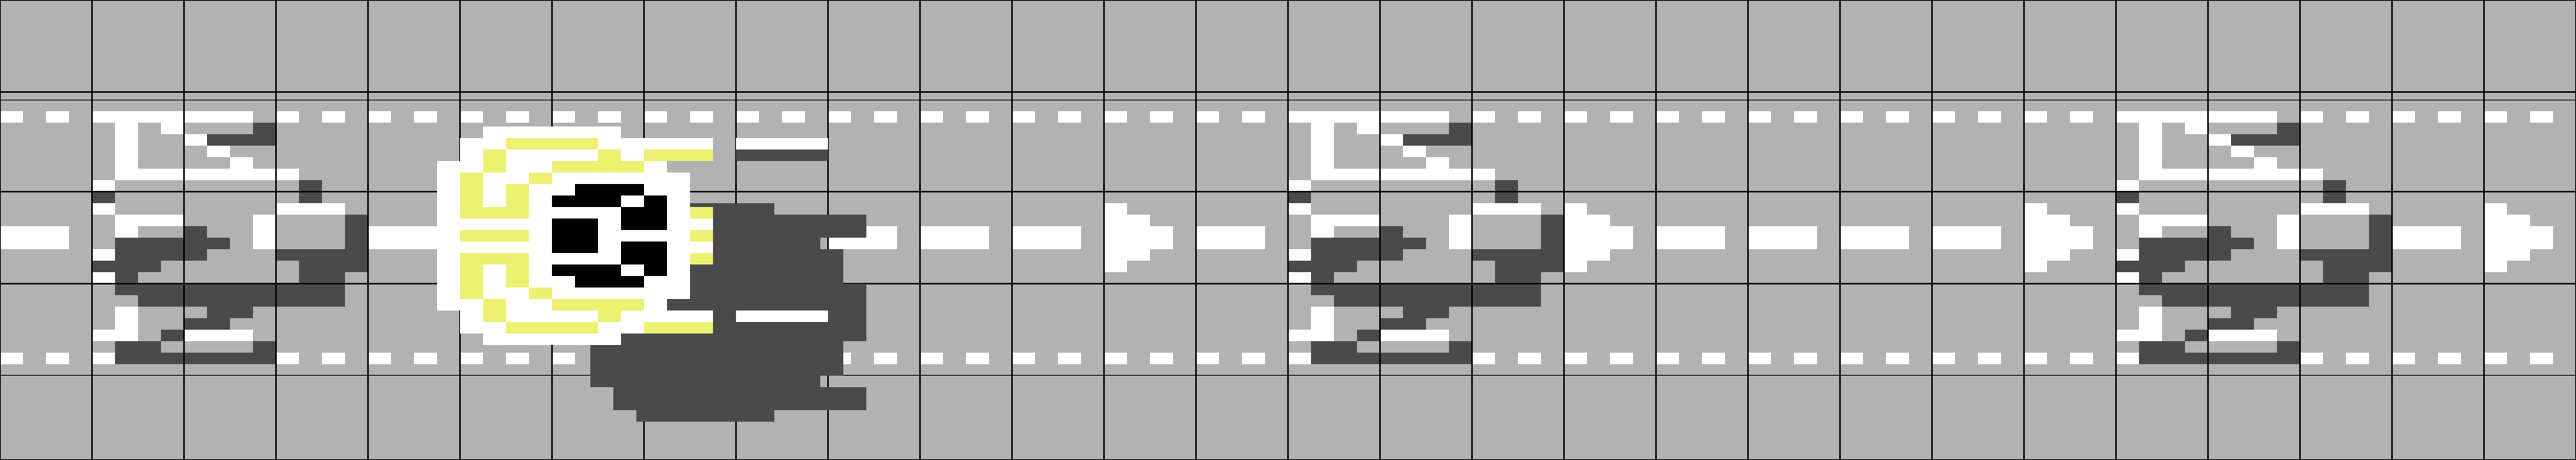
\includegraphics{src/bullets_player/level1_bullet_progress_64.png}%
    \end{adjustbox}
\end{figure}
\vspace{-0.4cm}

In the next frame, the bullet has made quite a bit of progress. We might have expected it to
advance by a single character width across the screen, instead it has advanced two whole character widths.
\begin{figure}[H]
    \begin{adjustbox}{width=13.2cm,left}
      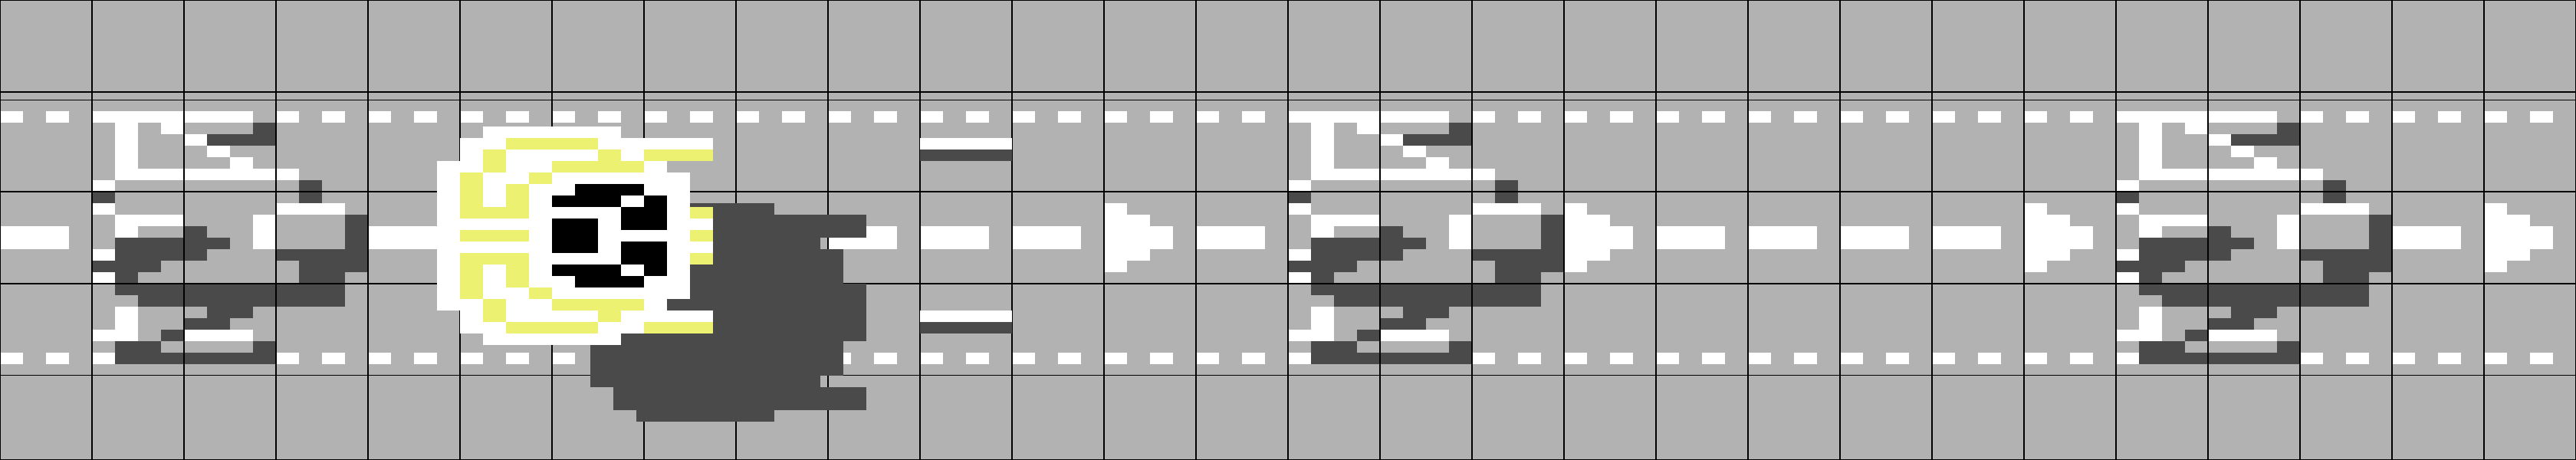
\includegraphics{src/bullets_player/level1_bullet_progress_80.png}%
    \end{adjustbox}
\end{figure}
\vspace{-0.9cm}
\begin{figure}[H]
    \begin{adjustbox}{width=13.2cm,left}
      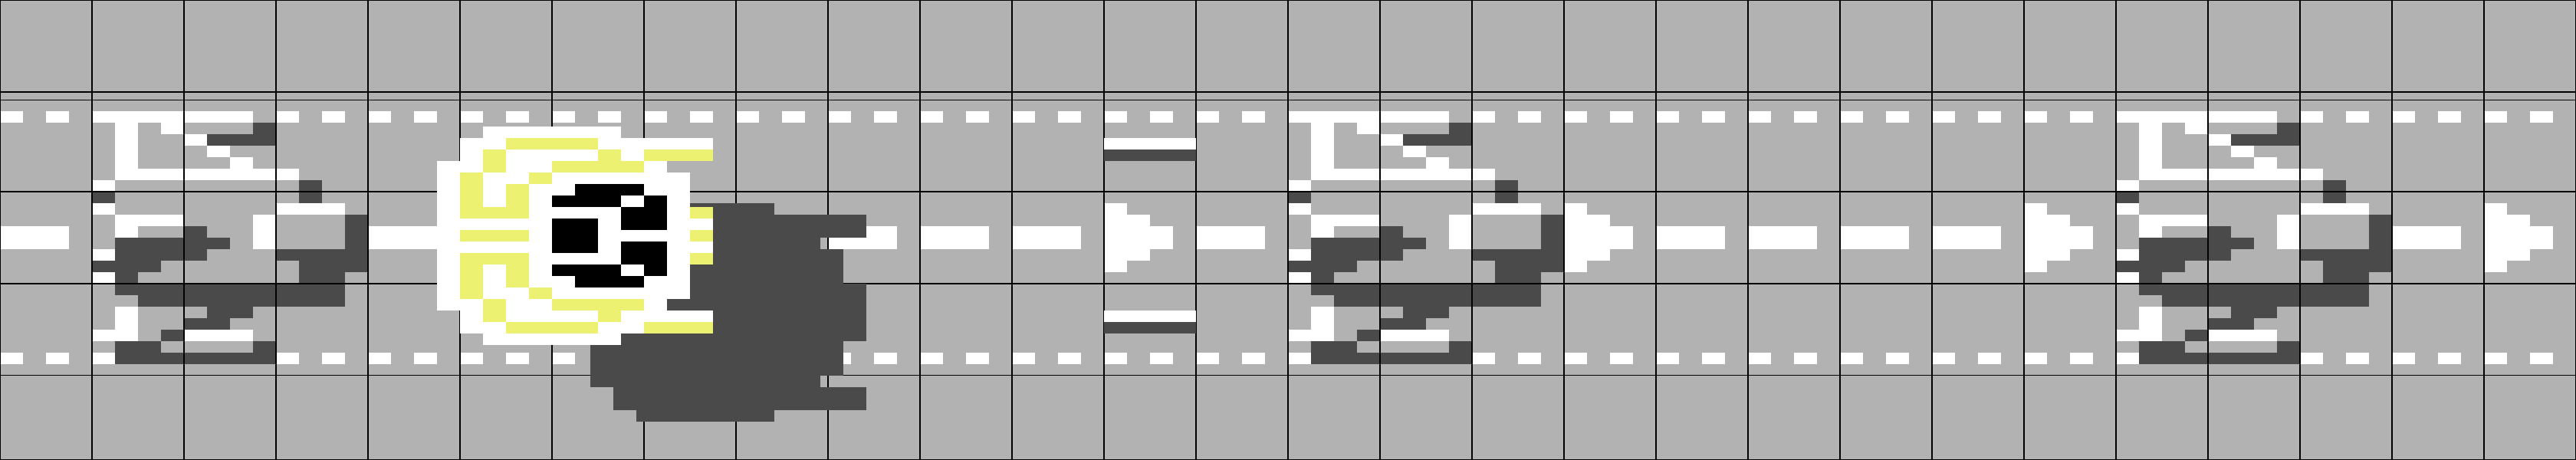
\includegraphics{src/bullets_player/level1_bullet_progress_96.png}%
    \end{adjustbox}
\end{figure}
\vspace{-0.4cm}

As the bullet continues to advance, we observe that this rate of progress was no fluke. The bullets
are advancing two characters at a time. The bullets are now on the verge of striking their target
on the deck. But before we discover the fate of their hapless victim, let's take stock of what we have
learned from this brief observation session.

Perhaps contrary to expectations, it would appear that the bullets are not sprites. They do not take
advantage of the pixel-perfect movement available to sprites, instead they move along character-width
boundaries. On short reflection, this approach makes sense. Bullets only ever travel laterally, there is
no complex movement required of them. They are also short-lived so we never have time to admire them or
their painstaking detail. Rendering bullets using the same character-based method adopted for the dreadnought's
surface starts to seem a natural choice when we contemplate their limited operation and duration. Lastly,
we can only ever display 8 sprites in a row at any given time. Since up to six bullets can be in flight at once,
we might not find ourselves with any capacity to display the Manta and its enemies if the available sprite slots
are already taken up by our bullets!

But this apparently clever economy of sprites comes with its own complexity cost. We must come up with a way
of compositing bullets onto the screen, rendering them over whatever is below (usually the surface of the dreadnought).
For example, the top bullet must be rendered by transforming the character below it: by drawing a white
and black line representing the bullet across the appropriate position of the character it is overlaying.
 
\begin{figure}[H]
    \centering
    \begin{adjustbox}{center}
      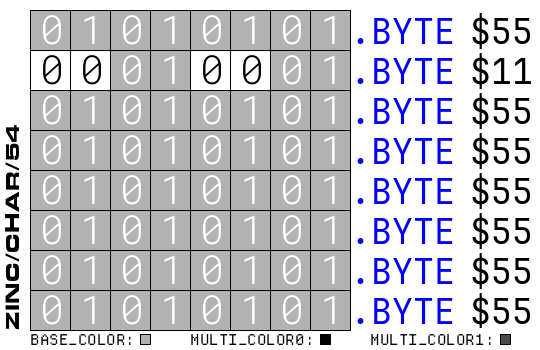
\includegraphics[width=6cm]{src/character_set_diagrams/1_54.png}%
      \hspace{0.2cm}
      \raisebox{2.5\totalheight}{
\includegraphics[height=0.6cm]{src/baydoor_sprites/arrow.png}}
      \hspace{0.2cm}
      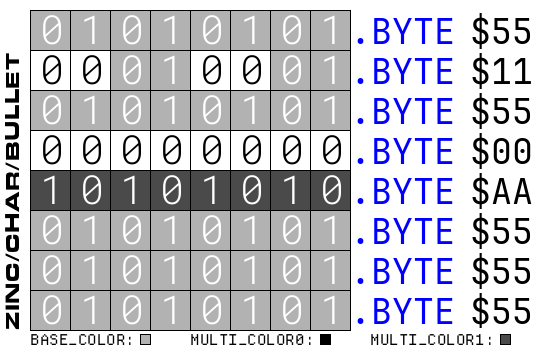
\includegraphics[width=6cm]{src/bullets_player/1_54_bullet.png}%
    \end{adjustbox}
\end{figure}
\vspace{-0.4cm}
Likewise for the bottom bullet, we must start with the character below, copy it, and then draw our bullet at the
appropriate vertical position.

\begin{figure}[H]
    \centering
    \begin{adjustbox}{center}
      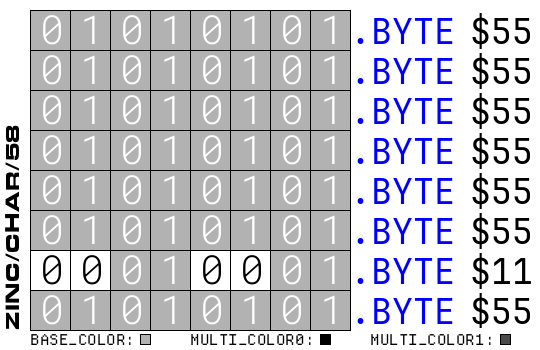
\includegraphics[width=6cm]{src/character_set_diagrams/1_58.png}%
      \hspace{0.2cm}
      \raisebox{2.5\totalheight}{
\includegraphics[height=0.6cm]{src/baydoor_sprites/arrow.png}}
      \hspace{0.2cm}
      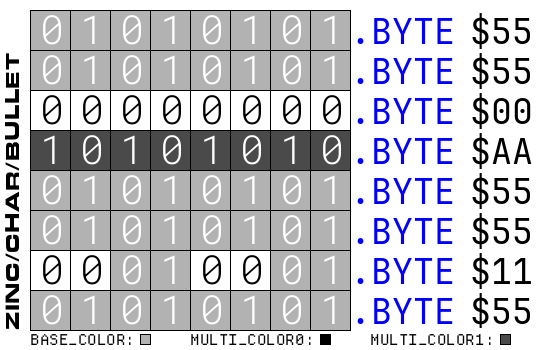
\includegraphics[width=6cm]{src/bullets_player/1_58_bullet.png}%
    \end{adjustbox}
\end{figure}
\vspace{-0.4cm}

The mechanics of this composition are relatively compact. Once we've identified the character definition
that specifies the background underneath the bullet's current position we copy its entire contents to
the bullet's character definition. This gives us our base.
\begin{lstlisting}
  LDY #$07                    ; We're copying all 8 lines of the character.
CharacterDefCopyLoop          
  LDA backgroundCharacter,Y   ; Load a line of character definition to A.
  STA (bulletCharDefLoPtr),Y  ; Copy it to our bullet character definition.
  DEY                         ; Decrement Y.
  BPL CharacterDefCopyLoop    ; Keep looping until Y reaches zero.
\end{lstlisting}

Next we draw our bullet over the top by adding in the bytes \icode{\$00} and \icode{\$AA} we see in our
diagrams above at the position that represents the vertical postion of the bullet within the character 'cell'.
\begin{lstlisting}
  LDY bulletOffsets,X         ; Get the vertical position of the bullet.
  LDA #$00                    ; The upper white line of the bullet.
  STA (bulletCharDefLoPtr),Y  ; Overwrite the background with it.
  INY                         ; Move down one line in the character.
  LDA #$AA                    ; The lower black line of the bullet.
  STA (bulletCharDefLoPtr),Y  ; Overwrite the background with it.
\end{lstlisting}

Now the question arises: what happens when the bullet actually hits something? And moreover,
how will we tell? Let's take a look at what happens when our bullet advances a final step
and finally overlaps some of the surface furniture.

\begin{figure}[H]
    \begin{adjustbox}{width=13.2cm,left}
      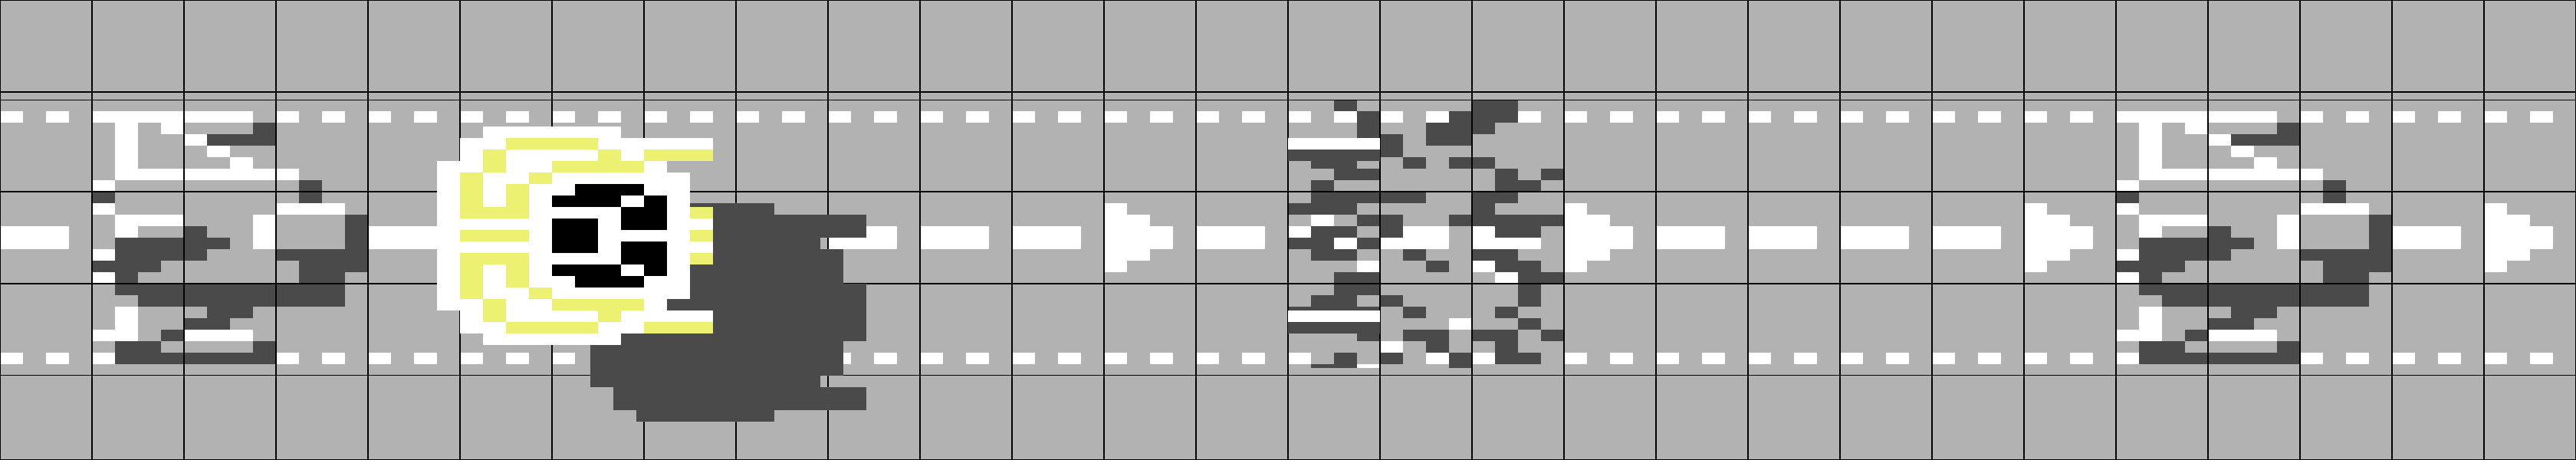
\includegraphics{src/bullets_player/level1_destroyed_bullet_progress_112.png}%
    \end{adjustbox}
\end{figure}
\vspace{-0.4cm}

It's the outcome we should expect. The answer to how we tell that the bullet has struck
this piece of surface lies once more in some careful selection of the values used to define the
features of the dreadnought's surface.

\begin{figure}[H]
    \begin{adjustbox}{width=13.2cm,left}
      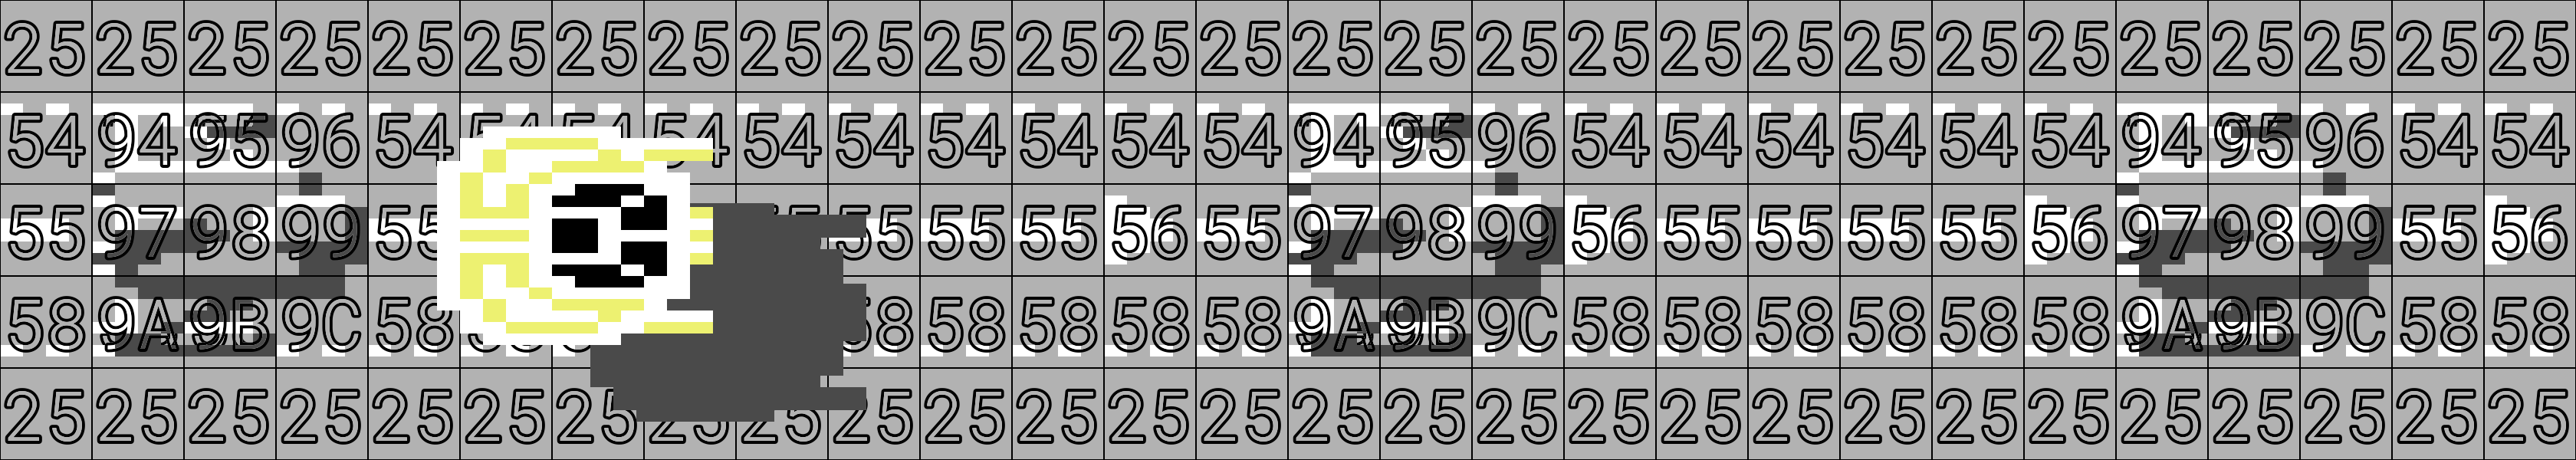
\includegraphics{src/bullets_player/level1_characters_bullet_progress_64.png}%
    \end{adjustbox}
\end{figure}
\vspace{-0.4cm}

We notice above that the characters used to specify the static enemy craft are all values between
\icode{\$94} and \icode{\$9C}. This is deliberate and in fact any character between \icode{\$90}
and \icode{\$9F} can be assumed to be part of a destroyable structure. Armed with this information,
we can detect a hit as follows:

\begin{lstlisting}
  LDA (ramLoPtr),Y      ; Get the character underneath the bullet.
  BPL DrawPlayerBullet  ; If it's less than $80, the bullet passes over.
  CMP #$90              ; If it's less than $90..
  BCC BulletBlocked     ; .. it blocks the bullet.
  CMP #$A0              ; If it's greater than $A0 ..
  BCS DrawPlayerBullet  ; .. the bullet passes over.
  ; If we get here the character is between $90 and $9F so..
  JSR DestroyStructure  ; .. the bullet destroys the structure!
\end{lstlisting}

Notice also that because our structures are always at least two characters wide, our bullets will
always detect a hit on something it can destroy, even though the bullets advance two characters at
a time. We avoid creating destroyable characters that are just one character wide because a bullet would always pass obliviously over them!


\begin{wrapfigure}[9]{r}{8cm} % <==========================================
\begin{minipage}[c]{0.40\linewidth}
      \vspace{-0.8cm}
\begin{figure}[H]
    \centering
\raisebox{-0.3\totalheight}{
\includegraphics[width=0.8cm]{src/character_mini_diagrams/1_94.png}}
\raisebox{-0.3\totalheight}{
\includegraphics[width=0.8cm]{src/character_mini_diagrams/1_95.png}}
\raisebox{-0.3\totalheight}{
\includegraphics[width=0.8cm]{src/character_mini_diagrams/1_96.png}}\\
\raisebox{-0.3\totalheight}{
\includegraphics[width=0.8cm]{src/character_mini_diagrams/1_97.png}}
\raisebox{-0.3\totalheight}{
\includegraphics[width=0.8cm]{src/character_mini_diagrams/1_98.png}}
\raisebox{-0.3\totalheight}{
\includegraphics[width=0.8cm]{src/character_mini_diagrams/1_99.png}}\\
\raisebox{-0.3\totalheight}{
\includegraphics[width=0.8cm]{src/character_mini_diagrams/1_9A.png}}
\raisebox{-0.3\totalheight}{
\includegraphics[width=0.8cm]{src/character_mini_diagrams/1_9B.png}}
\raisebox{-0.3\totalheight}{
\includegraphics[width=0.8cm]{src/character_mini_diagrams/1_9C.png}}
\end{figure}
\end{minipage}
\begin{minipage}[c]{0.08\linewidth}
      \vspace{-0.8cm}
\begin{figure}[H]
    \centering
    \begin{adjustbox}{center}
      \raisebox{1.2\totalheight}{
\includegraphics[height=0.4cm]{src/baydoor_sprites/arrow.png}}
    \end{adjustbox}
\end{figure}
\end{minipage}
\begin{minipage}[c]{0.40\linewidth}
      \vspace{-0.8cm}
\begin{figure}[H]
    \centering
\raisebox{-0.3\totalheight}{
\includegraphics[width=0.8cm]{src/character_mini_diagrams/1_74.png}}
\raisebox{-0.3\totalheight}{
\includegraphics[width=0.8cm]{src/character_mini_diagrams/1_75.png}}
\raisebox{-0.3\totalheight}{
\includegraphics[width=0.8cm]{src/character_mini_diagrams/1_76.png}}\\
\raisebox{-0.3\totalheight}{
\includegraphics[width=0.8cm]{src/character_mini_diagrams/1_77.png}}
\raisebox{-0.3\totalheight}{
\includegraphics[width=0.8cm]{src/character_mini_diagrams/1_78.png}}
\raisebox{-0.3\totalheight}{
\includegraphics[width=0.8cm]{src/character_mini_diagrams/1_79.png}}\\
\raisebox{-0.3\totalheight}{
\includegraphics[width=0.8cm]{src/character_mini_diagrams/1_7A.png}}
\raisebox{-0.3\totalheight}{
\includegraphics[width=0.8cm]{src/character_mini_diagrams/1_7B.png}}
\raisebox{-0.3\totalheight}{
\includegraphics[width=0.8cm]{src/character_mini_diagrams/1_7C.png}}
\end{figure}
\end{minipage}
\end{wrapfigure}
The business of actually destroying surface furniture is yet another case of carefully selected values.
If we have defined the shape of a destroyed structure using values with a common offset from the
values used to define the intact structure, we can perform a simple mapping or transformation like
the one opposite. In this case, subtracting \icode{\$20} from each character value to map it from
one in the range \icode{\$94} - \icode{\$9C} to one in the range \icode{\$74} - \icode{\$7C}. This
gives us the effect we are seeking and with relatively minimal coding required as we can see below,
where we simply inspect each character that makes up the structure and subtract \icode{\$20} from
it's value to refer to its destroyed version.
\clearpage

\begin{lstlisting}
DestroyStructureLoop
  LDY structureRAMIndex      ; Put the row location of the char in Y.
DestroyStructureRow
  LDA (structureRAMLoPtr),Y  ; Get the value of the character.
  CMP #$F0                   ; If it is greater than $F0..
  BCS GoToNextCharacter      ; .. then don't destroy it.
  SBC #$20                   ; Otherwise subtract $20..
  STA (structureRAMLoPtr),Y  ; .. and store it as the new value.
GoToNextCharacter
  DEY                        ; Go the next char in the row.
  BPL DestroyStructureRow    ; Until we're done with the row.

  DEC structureRAMIndex      ; Go the next row..
  BMI ExitDestroyLoop        ; Exit if it was the last.
  INC structureRAMHiPtr      ; Adjust the RAM Pointer to..
  INC structureRAMHiPtr      ; .. point to the next row.
  JMP DestroyStructureLoop   ; And 'destroy' the next row until done.
\end{lstlisting}
